% LaTeX Template for short student reports.
% Citations should be in bibtex format and go in references.bib
\documentclass[a4paper, 11pt]{article}
\usepackage[top=1cm, bottom=3cm, left = 2cm, right = 2cm]{geometry} 
\geometry{a4paper} 
\usepackage[utf8]{inputenc}
\usepackage{amsmath,amssymb}    
\usepackage[pdftex,bookmarks,colorlinks,breaklinks]{hyperref}  
%\hypersetup{linkcolor=black,citecolor=black,filecolor=black,urlcolor=black} % black links, for printed output
\usepackage[most]{tcolorbox}


\newtcolorbox{Summary}[1][]{
  enhanced,
  drop shadow={black!50!white},
  coltitle=black,
  top=0.1in,
  attach boxed title to top left=
  {xshift=1.5em,yshift=-\tcboxedtitleheight/2},
  boxed title style={size=small,colback=pink},
  title={#1}
}


\title{Distributed Key-Value Store in Akka}
\author{Fabrizio Sandri, Andrea Lorenzetti}

\begin{document}
\maketitle

\section{Introduction}

Inspired by Amazon Dynamo, this project introduces a DHT-based peer-to-peer key-value storage service implemented using Akka actors. It facilitates data upload, retrieval, and management commands while emphasizing key principles of data partitioning, replication, and dynamic network management.

Employing quorums and versioning, our system maintains consistency while accommodating read and write operations without breaking sequential consistency requirements. Additionally, it addresses dynamic network changes, such as node joins and leaves, with graceful data repartitioning. This report explores our architectural choices, demonstrating how our implementation fulfills the project's objectives of consistency and reliability within the context of modern distributed systems.

\section{Design choices}

In the actor-based Akka framework, the first step in our design process is to identify the key actors within the system. After careful analysis, it is clear that the system essentially requires two types of actors: client nodes and storage nodes. These nodes are created within the Main class and communicate exclusively through specific messages, as outlined in sections on Replication Messages \ref{Replication_Messages} and Repartitioning Messages \ref{Repartitioning_Messages}.

\paragraph{Main} The Main class serves as the central hub for managing the entire system. It reads incoming commands, processes them, and then dispatches the relevant message either to the client node (for join, get, or update requests) or to the storage node for operations like joining, leaving, crashing, or recovering.  

\paragraph{Client node} Client nodes have the capability to interact with any node within the storage network, either to retrieve an item or to request an item update. Additionally, they should be equipped to manage timeout errors resulting from unsuccessful requests.

\paragraph{Storage node} The essence of the entire system lies in its storage nodes, which encapsulate the project's fundamental logic. Unlike systems that require complex mechanisms like finger tables as seen in Chord, our system simplifies the process of locating the nodes responsible for a specific data item with key $k$. This is because each storage node is aware of every other node in the system, enabling local operations for data retrieval. To find the $N$ nodes responsible for a given key $k$, one can straightforwardly iterate through the storage node IDs, starting from the first node in the ring where the ID $I \geq k$. If no such node is found, it indicates that we have reached the end of the ring; in this case, the first $N$ nodes of the ring are returned. Otherwise, the remaining $N-1$ responsible nodes can be identified as those immediately following the first, with care taken to loop back to the start of the ring using modulo operations.

\subsection{Quorum based protocol}

In order to implement a sequentially consistency replicated storage system we have chosen to implement quorums based on the quorum based protocol proposed by Thomas (1979) and generalized by Gifford (1979). The essential principles of this protocol are as follows:
\begin{itemize}
    \item For read operations (both \textit{get} and \textit{read}), the coordinator node, which is selected by the client from the available nodes in the storage network, must contact $N$ replicas and obtain the response from at least $ R $ of them. This is to ensure that the most up-to-date version of a data item is obtained. Among the $ R $ versions retrieved, the most recent is guaranteed to be included.
    \item For write operations (both \textit{update} and \textit{write}), the coordinator needs to communicate with $ W $ replicas to acquire the most recent version of the data item. Once $ W $ confirmations are received, the system can ensure the latest version has been acquired and proceed to update the data item, thus establishing a write quorum.
\end{itemize}

It is vital to select appropriate values for $R$ and $W$ relative to $N$ to maintain system consistency. Specifically, the system must adhere to the following conditions:
\begin{enumerate}
    \item $R + W > N$ -- This condition is essential to avoid read-write conflicts. If both a read and a write operation occur simultaneously, this ensures that their quorums will intersect at least at one node. This guarantees the retrieval of the latest data version during the read operation.
    \item $W + W > N$ -- This is to prevent conflicts between two simultaneous write operations. Each of these write requests must form a write quorum with at least $ W_1 $ and $W_2$ nodes respectively. According to this rule, there will be at least one node common to both write quorums. This shared node will acknowledge only the first write request, causing the other to time out. It's also possible that none of the two write requests find a quorum and thus fall in deadlock, thus ensuring consistency.
\end{enumerate}



\subsection{Lock Management}
Simply adhering to the previously stated rules for setting $ R $ and $ W $ is not enough to guarantee sequential consistency. A mechanism must be in place to temporarily block access to specific items if doing otherwise would jeopardize the property of sequential consistency. We have chosen to implement a locking mechanism on individual items in the storage system. This ensures that when one node is modifying a key, other nodes are restricted from interacting with the corresponding item. The locking mechanism gives rise to three potential scenarios:

\begin{itemize}
    \item Concurrent read operations on a single key -- In this situation, both read operations can proceed safely without requiring any locks.
    
    \item A concurrent read and write on the same key -- The challenge here lies in the timing. The read operation could potentially acquire its read quorum before the write operation locks its $ W $ required replicas. In such a case, the read would complete successfully while the write is still in the process of acquiring locks. Conversely, if the write operation releases some of its locks after completing, and the read operation has already been initiated, the read quorum can still form successfully. Problems emerge when the write operation has already locked a majority of the $ N $ replicas, leaving fewer than $ R $ available. In such a situation, the read operation would time out as it cannot form its required read quorum.
    
    \item Concurrent write operations -- One write may succeed while the other fails due to missing quorums. This happens when one write operation manages to lock $ W $ different replicas, leaving only $ N-W $ replicas available. As the second protocol rule states $ W + W > N $, making it impossible for the second write operation to acquire $ W $ locks. Another potential outcome is deadlock, where both write operations time out. This scenario arises when all $ N $ replicas are locked, but neither of the two write operations has managed to secure a write quorum comprising $ W $ nodes. Both operations will consequently time out.
\end{itemize}

It's crucial to note that when a write request times out, all the locks it has obtained should be released. It's possible that other nodes might have simultaneously acquired locks on separate replicas for the same data item. To manage this case, we have designed a mechanism that uniquely associates each lock with a particular client. This enables the selective release of locks corresponding to a specific request from a given client, without affecting the locks secured by other requests.


\subsection{Replication messages}\label{Replication_Messages}
\begin{Summary}[Convention]
To reduce the chance of confusion due to terminology, we've opted to use the terms \textbf{update} and \textbf{get} for client-to-storage node communication. For interactions occurring between storage nodes themselves, we use the terms \textbf{write} and \textbf{read}.
\end{Summary}

\paragraph{Update operation} To better grasp how an update operates, let's delve into the messages exchanged between storage nodes and the client initiating the request:

\begin{enumerate}
    \item Update Request(\verb|updateRequestMsg|): This message is transmitted from the client to a storage node and contains the \textit{key} and \textit{value} of the item to be inserted into the DHT system.

    \item Write Request(\verb|WriteRequestMsg|): Once the storage node designated as the \textit{coordinator} receives the \verb|updateRequestMsg|, it contacts the $N$ replicas and informs them about the need for an update on a specific object identified by the \textit{key} in the message. This first write request is sent from the coordinator to all the $N$ replicas.

    \item Write Response(\verb|WriteResponseMsg|): The $N$ replicas receiving the previous message from the coordinator (the node initiating message exchange among storage nodes), check if the object's \textit{key} is already undergoing another update operation using the provided locking mechanism. If no concurrent write exists, the item is locked, and a write response which includes the \textit{version} of the item held by the node is sent back to the coordinator.

    \item Update Response(\verb|UpdateResponseMsg|): When the coordinator receives at least $W$ \verb|WriteResponseMsg| out of the $N$ replicas (ensuring the \textit{write quorum} is met), it sends a response to the client who initiated the request and to nodes awaiting confirmation of the update. This response includes the new \textit{value} and \textit{version} of the item. The client is now aware of the successful update. Upon receiving this message, storage nodes can update their replicas with the new \textit{version} and \textit{value} and release the lock for the specific key that has been updated.
\end{enumerate}

\paragraph{Get operation} Now that an update request has been made, any client may want to read the new version in the system. This can be accomplished using the \textit{get} request. Here is the series of message exchanges that occur, starting from the client to the storage nodes and then between the storage nodes:

\begin{enumerate}
    \item Get Request(\verb|GetRequestMsg|): The client node sends this message to a specific storage node, which, as seen in the update request, becomes the coordinator for this request. The message contains the \textit{key} that identifies the object.

    \item Read Request(\verb|ReadRequestMsg|): The coordinator receiving the get request first identifies the nodes that need to be contacted. It then sends to all the $N$ replicas a read request message with the object's \textit{key} to fetch their version of the item.

    \item Read Response(\verb|ReadResponseMsg|): Upon receiving the request, nodes check if the requested item is currently undergoing an update operation to avoid \textit{read-write conflicts}. If no issues arise, the \textit{value} is returned along with the \textit{version}, crucial for the coordinator. After collecting at least $R$ responses(to ensure a read quorum), the coordinator determines the most recent version of the items among the at least $R$ responses ensuring the \textit{sequential consistency} of the system.

    \item Get Response(\verb|GetResponseMsg|): After identifying the latest version of the item in question, the coordinator node forwards this most up-to-date version to the client that made the request.
\end{enumerate}

\begin{Summary}[Tracking requests]
As multiple requests may arrive simultaneously from different clients, each coordinator must keep track of received requests using a \textit{request ID}. By using the \textit{request ID}, the coordinator can efficiently match the response it receives from the storage nodes to the request from a client.
\end{Summary}

\paragraph{Timeouts} It's worth noting that these are not the only messages exchanged during requests. When the coordinator contacts other nodes for any of the described requests, it schedules a \verb|TimeoutMsg| message for itself. This safeguard accounts for situations where the quorum cannot be reached due to omitted responses from storage nodes that hold the item but are unable to respond because the item is already locked by another client's simultaneous write request.

\paragraph{Storage node crash} Users can send a \textit{crash} message to a storage node, making it unreachable for ordinary messages. It will only respond to a \textit{recovery} message sent by the user that will wake it up again and make it responsive to the ordinary messages. The crash message is a simple empty message that signals the node to become unavailable not only for update or get messages but also for leave and join operations, as described in the section \ref{Repartitioning_Messages} on Item repartitioning messages. Since the recovery of a storage node is tightly coupled to the join of a node, the recovery message will also be described in section \ref{Repartitioning_Messages}.

\subsection{Item repartitioning messages}\label{Repartitioning_Messages}

Item repartitioning in a DHT-system poses a complex challenge because the distribution of item replicas is constantly influenced by the dynamic nature of nodes that join and leave. In such a system, items are assigned to nodes according to particular guidelines. For this project, items—identified by keys—are spread across the first $N$ storage nodes, which have IDs equal to or greater than the key's value. This means that when a storage node joins or leaves, it can alter the distribution of keys.

\paragraph{Storage node join} When a user wants to add a new storage node to the network, they provide the new node's ID and a bootstrapping peer that assists the new node in connecting with the existing nodes. The process goes as follows:

\begin{enumerate}
    \item Join(\verb|JoinMsg|): This message is sent to the new storage node intending to join and contains the information about the bootstrapping peer to contact for necessary information.

    \item Get Set of Nodes(\verb|GetSetOfNodesMsg|): The new node sends this message to the bootstrapping peer to obtain the current list of nodes in the storage network.

    \item Set Of Nodes(\verb|SetOfNodesMsg|): The contacted peer responds with its list of nodes, enabling the new node to understand its position within the network topology and identify which storage node to contact for the items it should manage.

    \item Get Necessary Items(\verb|GetNecessaryItemsMsg|): After obtaining the list of nodes, the new storage node needs to contact its first clockwise neighbor to retrieve the keys and items it should store. The auxiliary function \verb|findClockWiseNeighbor| is used to determine the node to contact, and then this message is sent along with the joining node's ID. 

    \item  Necessary Item(\verb|NecessaryItemsMsg|): The neighbor responds with this message, providing the keys for which the new node is now responsible.

    \item Up To Date Item Request(\verb|UpToDateItemRequestMsg|): After receiving the list of keys, the new node aims to acquire the latest versions of these keys to ensure its storage is up-to-date. To accomplish this, it performs a read operation for all the necessary items, interacting with each of the $N$ replicas for the specific item.

    \item Up To Date Item Response(\verb|UpToDateItemResponseMsg|): When the previous request reaches the storage nodes, they respond with the value and version of the items they hold. This information is then sent back to the requester along with the key to track for which key the response is sent.

    \item Announce Join(\verb|AnnounceJoinMsg|): Once the minimum required responses (equivalent to a read quorum number of $R$ nodes) for each key are collected, the joining node stores the item with the latest version and its value. After adding the item, the new node introduces itself to the other storage nodes via a message containing its ID. When storage nodes receive the announcement message, they include the new storage node in their existing set of storage nodes. If they are holding items that are now stored in the new node, they eliminate those items to adhere to the rule of maintaining $N$ replicas.   

\end{enumerate}

It's important to note that in certain cases, nodes joining the network may not be able to complete this entire process. In such cases, they can directly announce their presence to all other storage nodes using the Announce Join message. These cases include:

\begin{itemize}
    \item When no other nodes are present in the network, preventing so to contact a bootstrap peer.
    \item When the number of nodes in the network is less than the minimum quorum number required to obtain item versions($R$). This case is designed to address the initial stages of the network. As highlighted in Section \ref{assumptions}, this feature should be employed solely during the network's early stages. For other situations, the first assumption explicitly mentions that if more than $N-R$ nodes fail, the read quorum cannot be achieved.
    \item When there are no items to be responsible for upon receiving the \verb|NecessaryItemsMsg|, allowing the joining node to announce its presence to the rest of the storage group without performing all the rest of the process.
\end{itemize}

\paragraph{Storage node leave} The node leaving process begins with a user command indicating the ID of the node that needs to leave the network. The messages that the storage node must handle are as follows:

\begin{enumerate}
    \item Leave Message(\verb|LeaveMsg|): This message originates from the user and is sent directly to the storage node that is exiting the system. This node identifies which other storage nodes will take over its responsibilities and sends them an \verb|AnnounceLeaveMsg| containing the items they should now manage. The \verb|findNodesForKey| function iterates through all the items in the storage of the departing node to identify the node that should take responsibility for each specific item. This ensures that data is only transferred to the nodes that are actually responsible for it.
    \item Announce Leave Message(\verb|AnnounceLeaveMsg|): This message includes the ID of the node that is leaving and specifies the new items that a receiving storage node should take over. Upon receiving this message, storage nodes remove the departing node's ID from their list of recognized storage nodes. If the list of items to take responsibility for is not empty, they integrate these new items into their existing storage.
\end{enumerate}

\paragraph{Storage node recovery} The recovery process from a crash follows a similar message exchange flow as the joining process. This is because when a node crashes, it essentially disappears from the network until it receives a recovery message, requiring it to retrieve updates from other nodes in the storage network. As with the other processes, recovery originates from a user command specifying the node to recover and a bootstrapping peer (similar to joining). For completeness and consistency, here are the messages exchanged during a recovery process:

\begin{enumerate}
    \item Recovery Message(\verb|RecoveryMsg|): This message signals to the crashed node that it must recover and resume responding to the system's regular messages. Upon handling this message, a new \verb|GetSetOfNodesMsg| is sent to the bootstrapping peer. The procedure then proceeds similarly to the standard joining process, except that the join announcement message is not dispatched.
\end{enumerate}

It's important to consider that since the message handlers for a recovery process and a joining process are the same, mechanisms were implemented to distinguish between the two processes. This ensures that certain actions are triggered only during a join or a recovery. This separation was necessary to prevent incorrect behavior during either process.

\section{Implementation details}


Our project architecture consists of the following Java classes:
\begin{itemize}
    \item \verb|Main.java|: Serving as the application's entry point, this class primarily focuses on command interpretation. The function \verb|parseCommand| is responsible for executing received commands. We realized the utility of loading initial commands from a pre-defined text file, named \verb|commands.txt|, when the application starts. Subsequent commands are processed from the command line.
    \item \verb|StorageNode.java|: This class constitutes the backbone of the storage network. Further particulars concerning its implementation are elaborated in section \ref{storage_node}.
    \item \verb|ClientNode.java|: Represents the client-side node and is tasked with issuing update and get requests to the storage network.
    \item \verb|Item.java|: Represents a data item in the key-value storage. It contains attributes like value and version, along with a Boolean variable to indicate the item's lock status.
\end{itemize}


\subsection{Storage node}\label{storage_node}

This class serves as the backbone of the entire project, and we'd like to briefly discuss its key variables. Although each variable is commented in the code for further clarification, we particularly want to spotlight the following critical ones.

\begin{itemize}
    \item \verb|Map<Integer, ActorRef> storageNodes|: This map lists all the storage nodes in the network. Any storage node can fetch the $ActorRef$ of another node by using its key to query this map.
    \item \verb|Map<Integer, Item> storage|: This map serves as the node's local storage facility, in line with the requirements of the assignment, thus providing a persistent storage mechanism.
    \item \verb|int requestId|: This variable keeps track of the number of incoming requests from clients. It is used to differentiate between various requests. Each time a \textit{get} or \textit{update} request is made to this node, the \verb|requestId| is incremented.
    \item \verb|Map<Integer, ActorRef> lockedBy|: This map keeps a record of which actor has initiated a lock on an item, thereby preventing any unauthorized actor from unlocking it.
    \item \verb|Map<Integer, List<Item>> quorum|: This variable stores items received from requests based on their request IDs. It is used for both selecting the latest version of items for a specific \verb|requestId| and for checking if quorum conditions are satisfied for that \verb|requestId|.
\end{itemize}

\paragraph{Simulating storage nodes Crash and Recovery} Upon getting \verb|CrashMsg|, a storage node mimics its own failure by altering the Akka actor's actions through \verb|getContext().become(crashed())|. In this crashed state, the node solely responds to a \verb|RecoveryMsg|. Upon receipt of this message, the node once again modifies its behavior to emulate recovery, utilizing \verb|getContext().become(createReceive())|.


\paragraph{Delays} In distributed systems, communication delays can occur due to network traffic or slow host connections. Since the Akka framework does not inherently simulate these potential delays, we have incorporated artificial delays using the \texttt{Thread.sleep} function. This allows us to intentionally introduce delays during our testing sessions, thereby exerting more stress on our system for testing purposes.

\subsection{Illustrative Example}
This section offers an illustrative example aimed at explaining the functioning of the entire architecture. Assume a scenario as shown in Figure \ref{example}, where $N=3$, $R=2$, and $W=2$. Also, consider that two different clients wish to update the item associated with key $13$, but with different values. For clarity, each message is numbered based on its execution order.

\begin{figure}[htb]
\begin{center}
\label{example}
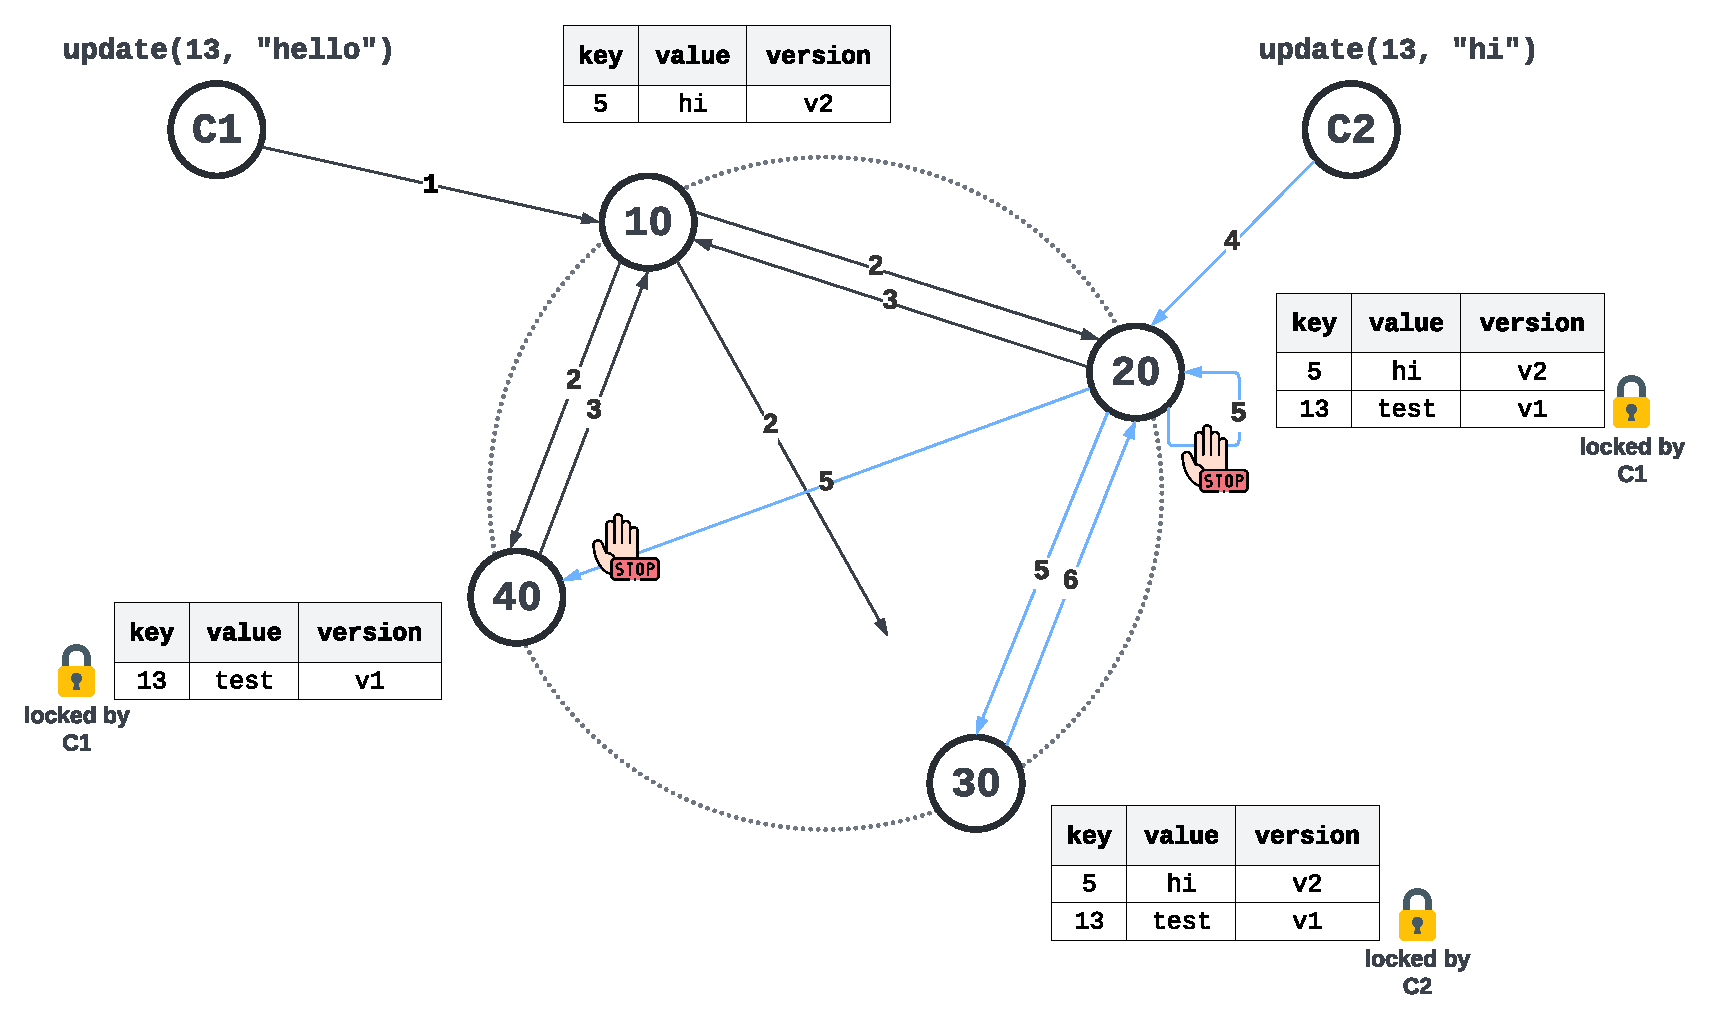
\includegraphics[height=3.5in]{example.pdf}
\caption{Example of how the system handles write-write conflicts on the same item key.}
\end{center}
\end{figure}

\begin{enumerate}
    \item Initially, client $C1$ sends an \verb|updateRequestMsg| that includes both the key and value for the item to be updated, targeting storage node $10$ as the coordinator.
    \item On receiving this, node $10$ designates a unique identifier for the incoming request, enabling the correlation of subsequent requests to the originating client's query. The coordinator then communicates with the $N$ replicas by sending them a \verb|WriteRequestMsg|.
    \item Assume at this stage that two out of the three total replicas have successfully received the \verb|WriteRequestMsg|. Meanwhile, the message to node $30$ is still in transit. Nodes $20$ and $40$, upon confirming that the key $13$ is not currently locked, secure it. They indicate this status using the boolean variable \verb|lock| on the item and using the \verb|lockedBy| map and reply to the coordinator with a \verb|WriteResponseMsg|. The coordinator, now with a write quorum secured, could issue an \verb|UpdateResponseMsg| to notify both the client and the storage nodes about the update. For the purpose of this example, however, consider that a second client $C2$ initiates a concurrent update on the same key before the \verb|UpdateResponseMsg| is sent.
    \item In a similar fashion to $C1$, client $C2$ transmits an \verb|updateRequestMsg| for the same key $13$, but with a distinct value, selecting node $20$ as the coordinator.
    \item The second request's coordinator sends out the \verb|WriteRequestMsg| to all $N$ replicas. Unfortunately, two replicas find the item with key $13$ already locked due to $C1$'s request, resulting in no response from nodes $20$ and $40$. Conversely, node $30$ receives $C2$'s \verb|WriteRequestMsg| before the one from $C1$, locks the item, and sends back a \verb|WriteResponseMsg|. As only one reply is received by coordinator $20$, $C2$'s request times out after $T$ seconds, automatically releasing any locks it had acquired. $C2$ is then notified of the timeout via an error message.
\end{enumerate}

Though the update from $C2$ is unsuccessful, $C1$'s request completes by sending an \verb|UpdateResponseMsg| to both the client and the replicas. Once the replicas receive this message, they perform the item update and release the associated lock.



\section{Assumptions}\label{assumptions}
In the final section, we outline the supplementary assumptions that are essential for the correct functioning of the entire project.
\begin{itemize}
    \item For any data item within the storage network, the maximum number of nodes that may crash is $N-R$. This ensures that during node recovery or join into the network, a read quorum comprising at least $R$ nodes can be established to retrieve the missing items; failing this, the recovery or join processes would fail.
    \item Should the number of storage nodes be precisely $N$, no additional node can exit the network. Leaving under these conditions would make it impossible for the leaving node to delegate its keys to another node.
    \item A storage node identified by ID $i$ will hold the key $k$ if $i = k$. This guarantees that the key $k$ is retained in the following $N$ nodes, starting with node $k$ itself.
\end{itemize}

\end{document}
